\begin{frame}{Natural Language Need}
	\begin{itemize}\setlength\itemsep{3em}
		\item Natural Language $\neq$ Protein Sequences
		\begin{itemize}\setlength\itemsep{1em}
			\item Natural language is \underline{complete} for NLP tasks
			\begin{itemize}
				\item Natural language can represent all \emph{components} for NLP tasks
				\\$\cdot$ \emph{components}: input instructions, expected output
			\end{itemize}
			\item Protein language is \underline{NOT complete} for PLP tasks
		\end{itemize}
		\item Example: protein property prediction task
		\begin{itemize}
			\item task instruction: ``Predict the property of this protein: MAFCF...FEV''
			\item expected output: ``The property is Trx superfamily.''
		\end{itemize}
	\end{itemize}
\end{frame}

\begin{frame}{Natural Language Ability}
	\begin{center}
		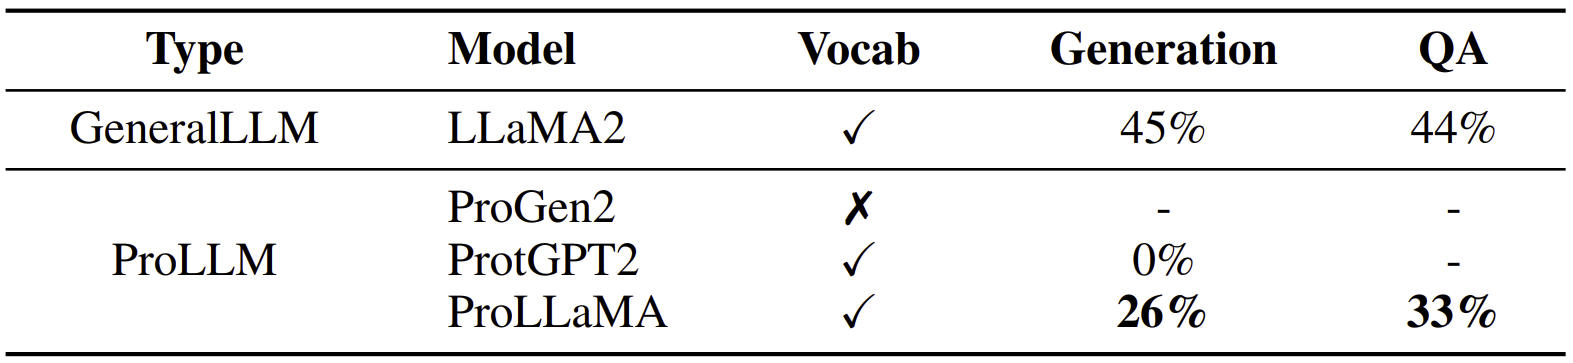
\includegraphics[scale=0.21]{tables/natural_language_ability_comparison.png}
	\end{center}
	\credit{Table}{lv2024prollama}
	\begin{itemize}
		\item Sentence generation on Wikipedia text
	\end{itemize}
\end{frame}